%%%%%%%%%%%%%%%%%%%%%%%%%%%%%%%%%%%%%%%%%%%%%%%%%%%%%%%%%%%%%%%%%%%%%%%%%%%%%%%%
% TUM-Vorlage: Präsentation - Beispiele
%%%%%%%%%%%%%%%%%%%%%%%%%%%%%%%%%%%%%%%%%%%%%%%%%%%%%%%%%%%%%%%%%%%%%%%%%%%%%%%%


\begin{frame}
\frametitle{The Cell Data-Structure - Approach 1}
\large
Idea:
\vspace{-0.5cm}
\begin{itemize}
	\item Sort Particles in accordance to their Cell Position
	\item save which part of the particles-Vector corresponds to which cell
\end{itemize} 

%\resizebox{0.5\textwidth }{0.5\textheight }{
	\begin{tikzpicture}
	%define constants
	\def\offGrid{3.5}
	\def\offP{2.5}
	\def\arrowStart{0.6}
	\def\arrowEnd{1.9}
	
	\def\scale{1.4}
		
	%draw grid scetch
	\foreach \k in {0,...,3} {
		\draw (\scale*\offGrid+\scale*\k,\scale*0)--(\scale*\offGrid+\scale*\k,\scale*3);
		\draw (\scale*\offGrid +\scale*0,\scale*\k)--(\scale*\offGrid+\scale*3,\scale*\k);
	}

	\node[] at (\scale*\offGrid+\scale*0.3, \scale*1.2) {p0};
	\node[] at (\scale*\offGrid+\scale*1.6, \scale*1.2) {p1};
	\node[] at (\scale*\offGrid+\scale*1.3, \scale*1.6) {p2};

	%draw datastructure scetch
	
	%particle vector
	\foreach \k in {0,...,2} {
		\node[fill=gray] at (\scale*\offP, \scale*2+\scale*0.5-\scale*\k) {p$\k$};
	}
	\node at (\scale*\offP, -\scale*0.6) {particles.end()};
	
	\node[] at (\scale*\offP, +\scale*3.5) {particles};

	%cells
	\node[] at (\scale*0, +\scale*3.5) {cells};

	\node[] at (\scale*0, \scale*2.6 + \scale*0.5) {\vdots};
	\node[] at (\scale*0, \scale*2 + \scale*0.5) {Cell 3};
	\node[] at (\scale*0, \scale*1 + \scale*0.5) {Cell 4};
	\node[] at (\scale*0, \scale*0 + \scale*0.5) {Cell 5};
	\node[] at (\scale*0, \scale*-0.4 + \scale*0.5) {\vdots};
	
	%arrows
	\draw[-triangle 60] (\scale*\arrowStart, \scale*2 + \scale*0.5) -- (\scale*\arrowEnd, \scale*2 + \scale*0.5);
	
	\draw[-triangle 60] (\scale*\arrowStart, \scale*1 + \scale*0.5) -- (\scale*\arrowEnd, \scale*1 + \scale*0.5);
	
	\draw[-triangle 60] (\scale*\arrowStart, \scale*0 + \scale*0.5) -- (\scale*\arrowEnd, -\scale*0.8 + \scale*0.5);
	
	\end{tikzpicture}
%}

\end{frame}

\begin{frame}
	\frametitle{The Cell Data Structure - Approach 2}
	\large
	Idea:
	
	Approach 1.1 stored multiple virtual vectors in one vector $\rightarrow$ let's actually store the particles in vectors corresponding to their cell

	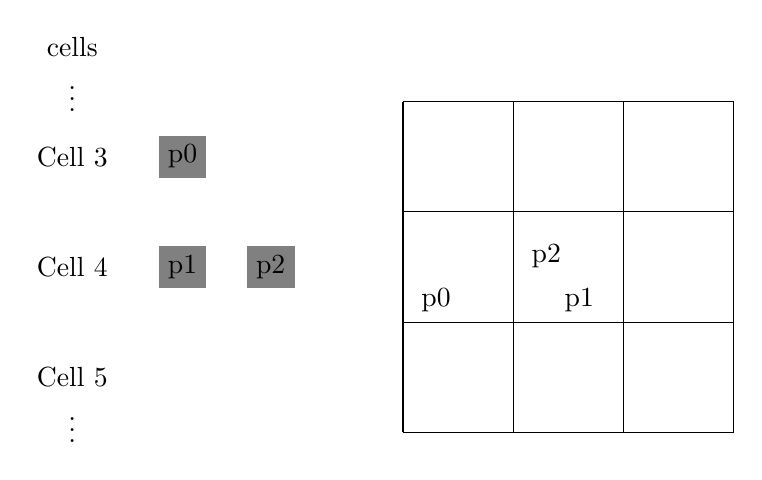
\begin{tikzpicture}
		%define constants
		\def\offGrid{3}
		\def\offP{2.5}
		\def\arrowStart{0.6}
		\def\arrowEnd{1.9}
		
		\def\scale{1.4}
		
		%draw grid scetch
		\foreach \k in {0,...,3} {
			\draw (\scale*\offGrid+\scale*\k,\scale*0)--(\scale*\offGrid+\scale*\k,\scale*3);
			\draw (\scale*\offGrid +\scale*0,\scale*\k)--(\scale*\offGrid+\scale*3,\scale*\k);
		}
		
		\node[] at (\scale*\offGrid+\scale*0.3, \scale*1.2) {p0};
		\node[] at (\scale*\offGrid+\scale*1.6, \scale*1.2) {p1};
		\node[] at (\scale*\offGrid+\scale*1.3, \scale*1.6) {p2};
		
		%draw datastructure scetch
		
		%cells
		\node[] at (\scale*0, +\scale*3.5) {cells};
		
		\node[] at (\scale*0, \scale*2.6 + \scale*0.5) {\vdots};
		
		\node[] at (\scale*0, \scale*2 + \scale*0.5) {Cell 3};
		\node[fill=gray] at (\scale*1, \scale*2+\scale*0.5-\scale*0) {p0};
		
		\node[] at (\scale*0, \scale*1 + \scale*0.5) {Cell 4};
		\node[fill=gray] at (\scale*1, \scale*2+\scale*0.5-\scale*1) {p1};
		\node[fill=gray] at (\scale*1.8, \scale*2+\scale*0.5-\scale*1) {p2};
		
		\node[] at (\scale*0, \scale*0 + \scale*0.5) {Cell 5};
		\node[] at (\scale*0, \scale*-0.4 + \scale*0.5) {\vdots};
	
		
	\end{tikzpicture}
\end{frame}

\begin{frame}
\frametitle{The Cell Data Structure - Approach 3}
	\large
	Idea:
	\vspace{-0.5cm}
	\begin{itemize}
		\item Each Cell only keeps references to their members
		\item No sorting or copying of entire particles required
	\end{itemize} 
	
	%\resizebox{0.5\textwidth }{0.5\textheight }{
		\begin{tikzpicture}
			%define constants
			\def\offGrid{3.5}
			\def\offP{2.5}
			\def\arrowStart{0.6}
			\def\arrowEnd{1.9}
			
			\def\scale{1.4}
			
			%draw grid scetch
			\foreach \k in {0,...,3} {
				\draw (\scale*\offGrid+\scale*\k,\scale*0)--(\scale*\offGrid+\scale*\k,\scale*3);
				\draw (\scale*\offGrid +\scale*0,\scale*\k)--(\scale*\offGrid+\scale*3,\scale*\k);
			}
			
			\node[] at (\scale*\offGrid+\scale*0.3, \scale*1.2) {p0};
			\node[] at (\scale*\offGrid+\scale*1.6, \scale*1.2) {p1};
			\node[] at (\scale*\offGrid+\scale*1.3, \scale*1.6) {p2};
			
			%draw datastructure scetch
			
			%particle vector
			\foreach \k in {0,...,2} {
				\node[fill=gray] at (\scale*\offP, \scale*2+\scale*0.5-\scale*\k) {p$\k$};
			}
			%\node at (\scale*\offP, -\scale*0.6) {particles.end()};
			
			\node[] at (\scale*\offP, +\scale*3.5) {particles};
			
			%cells
			\node[] at (\scale*0, +\scale*3.5) {cells};
			
			\node[] at (\scale*0, \scale*2.6 + \scale*0.5) {\vdots};
			\node[] at (\scale*0, \scale*2 + \scale*0.5) {Cell 3};
			\node[] at (\scale*0, \scale*1 + \scale*0.5) {Cell 4};
			\node[] at (\scale*0, \scale*0 + \scale*0.5) {Cell 5};
			\node[] at (\scale*0, \scale*-0.4 + \scale*0.5) {\vdots};
			
			%arrows
			\draw[-triangle 60] (\scale*\arrowStart, \scale*2 + \scale*0.5) -- (\scale*\arrowEnd, \scale*2 + \scale*0.5);
			
			\draw[-triangle 60] (\scale*\arrowStart, \scale*1 + \scale*0.5) -- (\scale*\arrowEnd, \scale*1 + \scale*0.5);
			
			\draw[-triangle 60](\scale*\arrowStart, \scale*1 + \scale*0.5) -- (\scale*\arrowEnd, + \scale*0.5);
			
			%\draw[-triangle 60] (\scale*\arrowStart, \scale*0 + \scale*0.5) -- (\scale*\arrowEnd, -\scale*0.8 + \scale*0.5);
			
		\end{tikzpicture}
	
\end{frame}

\begin{frame}
	\frametitle{Approach Comparison}
	\large
	\setlength\tabcolsep{0.5cm}
	\def\arraystretch{1.5}
	\begin{tabularx}{\linewidth}{>{\hsize=.33\hsize}X|>{\hsize=.33\hsize}X|>{\hsize=.33\hsize}X}		
		
		Approach 1 & Approach 2 & Approach 3 \\
		\hline
		\textcolor{black}{$+$ Easy to implement} & 
		\textcolor{black}{$+$ Easy to implement} &
		\textcolor{black}{$+$ Easy to implement} \\ 
		
		
		
		\textcolor{black}{$+$ Interface for old Assignments remains unchanged} & 
		\textcolor{black}{$+$ New Implementation of some methods needed} &
		\textcolor{black}{$-$ Interface for old Assignments remains unchanged} \\
		
		\textcolor{black}{$-$ Expensive struct swaps during sorting} & 
		\textcolor{black}{$-$ Expensive struct copies with potential reallocs needed} &
		\textcolor{black}{$+$ References are cheap} \\
		
		\textcolor{black}{$+$ Direct access to particles for calculations} & 
		\textcolor{black}{$+$ Direct access to particles for calculations}&
		\textcolor{black}{$+$ Dereferencing needed} \\		
	\end{tabularx}

	\pause
	\vspace{0.4cm}
	In the end we decided to implement approach 3.
¸\end{frame}

\begin{frame}[fragile]
	\frametitle{Spheres}
	\large
	Expansion of the Body-struct utilized in Assignment 2
	
	\begin{columns}
		
	\begin{column}{0.48\textwidth}
	\begin{lstlisting}[language=C++]	
enum Shape {cuboid, sphere};
struct Body {
	Shape shape;   
	Eigen::Vector3d fixpoint; 
	Eigen::Vector3d dimensions;
	double distance;
	double mass;
	Eigen::Vector3d start_velocity;
} ;
	\end{lstlisting}	
	\end{column}

	\begin{column}{0.48\textwidth}
		\vspace{-1.5cm}
		\begin{equation*}
			\begin{aligned}
				\sqrt{x^2 + y^2 + z^2} & <= r\\
				\iff x^2 + y^2 + z^z   & <= r^2
			\end{aligned}
		\end{equation*}
	
		\vspace{0.5cm}
		
		\begin{center}
			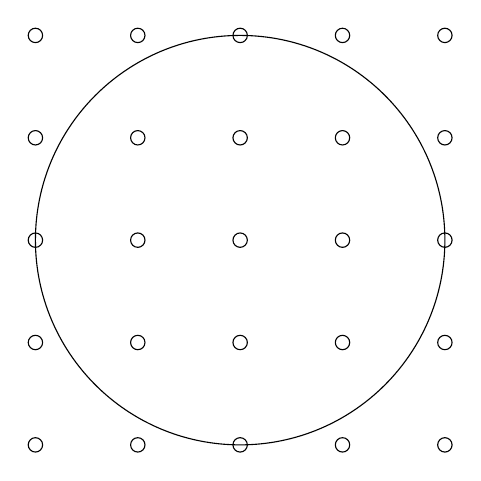
\begin{tikzpicture}[scale=1.3]
				\foreach \x in {0,...,4}{
					\foreach \y in {0,...,4}{
						\draw (\x, \y) circle[radius=2pt];
					}
				}
				
				\draw (2,2) circle[radius=2];
				
				
			\end{tikzpicture}
		\end{center}
	\end{column}

\end{columns}
	
\end{frame}

\begin{frame}[fragile]
	\frametitle{ParticleContainer's new methods}
	\vspace{0.4cm}
	
	\begin{lstlisting}[language=C++]
class ParticleContainer{
	...

	void forAllPairsInSameCell(void (*fun) (Particle& p1, Particle& p1));
	
	void forAllPairsInNeighbouringCell(void (*fun) (Particle& p1, Particle& p1));
	
	void forAllCells(void (*fun)(...));
	
	void forAllDistinctNeighbouringCells(void (*fun) (...));
		
	...
}
\end{lstlisting}

	\large

\begin{itemize}
	\item Functionality of first two methods is sufficient but hard to optimize
	\item Functionality of last two methods results in higher cohesion, but potential for runtime improvement
\end{itemize}
	
\end{frame}

\begin{frame}
	\frametitle{}
	

\end{frame}


\begin{frame}
	\frametitle{IO}

	\large
	\centering
	input Loader gets chosen at compile time
	%\begin{itemize}
	%\item inputLoader gets chosen at compile time
	%\end{itemize}
\end{frame}


\begin{frame}[fragile]
\frametitle{Input parsing - Definition of Body}
\vspace{0.7cm}

\begin{lstlisting}[language=C++]
enum Shape {cuboid, sphere};

struct Body {
	Shape shape;   
	Eigen::Vector3d fixpoint; 
	Eigen::Vector3d dimensions; 
	double distance;
	double mass;
	Eigen::Vector3d start_velocity;
} ;
\end{lstlisting}
\end{frame}

\begin{frame}
	\frametitle{CI/CD}
	\large
	\begin{itemize}
		\item<1-> Protection of master branch
		\item<2-> Deployment of CI/CD pipeline for \textit{all} branches 
	\end{itemize}
	
\end{frame}


\begin{frame}
	\frametitle{CI/CD}
	\large
	\begin{itemize}
		\item Protection of master branch
		\item Deployment of CI/CD pipeline for \textit{all} branches 
	\end{itemize}
	\Large
	The pipeline consist of:
	\large
	\begin{itemize}
		\item<1-> library installation
		\item<2-> build process
		\item<3-> sanitizers
		\item<4-> unit tests for every major component
	\end{itemize}
\end{frame}

\begin{frame}[fragile]
	\frametitle{CI/CD}
	\begin{lstlisting}
		name: Build and Gtest
		on:
		push:
		branches:
		- '**'        # matches every branch
		pull_request:
		branches: ["master"]
		env:
		#Customize CMake build type here from [Debug;Release;RelWithDebInfo;MinSizeRel]
		BUILD_TYPE: Release	
	\end{lstlisting}
\end{frame}

\begin{frame}[fragile]
	\frametitle{Logging}
	\large
	format:
	\begin{lstlisting}
		[time][level::context] message
	\end{lstlisting}
	
	
	\begin{itemize}
		\item 6 different log-levels available
		\item log-level can be chosen via command line input
		\item use of log functions since we don't log in performance critical areas
		\item no need to deactivate logging at compile time
	\end{itemize}
\end{frame}

\begin{frame}
	\frametitle{Performance optimization - "Gaussian multithreading"}
	\vspace{1.5cm}
	\begin{columns}
		\begin{column}{0.48\textwidth}
	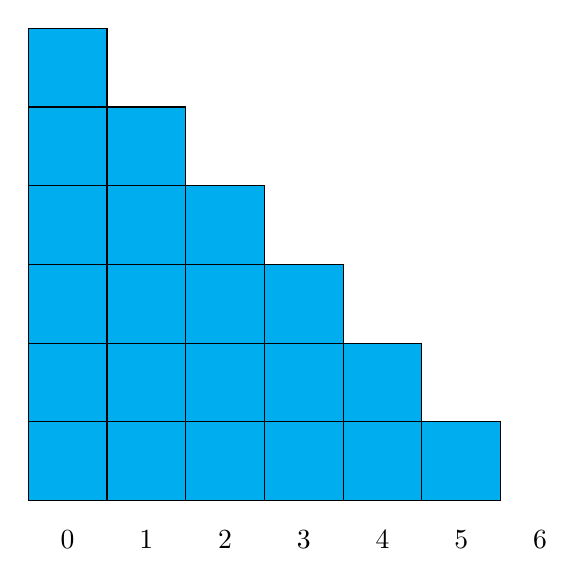
\begin{tikzpicture}
		\foreach \x in {0,...,5}
		\foreach \y in {0,...,\x} 
		\filldraw[draw=black,fill=cyan] (5-\x,\y) rectangle (5-\x+1,\y+1);
		\foreach \k in {0,...,6} {
			\node[] at (\k+0.5, -0.5) {$\k$};
		}	
	\end{tikzpicture}
		\end{column}
		\begin{column}{0.48\textwidth}
	\vspace{-6.5cm}
	\large
	\begin{itemize}
	\item Idea: Force calculation can be multithreaded quite easily 
	\item Evenly distribute Particle-pairs among multiple threads \\
	\item One rectangle represents one necessary force-calculation where $\min(p1,p2)$ is the number displayed below
	\end{itemize}
		\end{column}
	\end{columns}	
\end{frame}

\begin{frame}
	\frametitle{Performance optimization - "Gaussian multithreading"}
		\vspace{1.5cm}
		\begin{columns}
		\begin{column}{0.48\textwidth}
			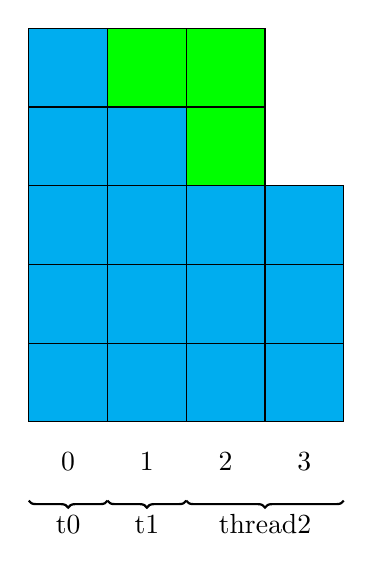
\begin{tikzpicture}
	\foreach \x in {0,...,2}
		\foreach \y in {0,...,2} 
			\filldraw[draw=black,fill=cyan] (\x,\y) rectangle (\x+1, \y+1);
	\foreach \k in {0,...,3} {
		\node[] at (\k+0.5, -0.5) {$\k$};
	}	
	\foreach \x in {0,...,2}
		\foreach \y in {0,...,\x} 
			\filldraw[draw=black,fill=cyan] (2-\x,\y+2) rectangle (2-\x+1, \y+1+2);
	\filldraw[draw=black,fill=green] (1,4) rectangle (2,5);
	\filldraw[draw=black,fill=green] (2,4) rectangle (3,5);
	\filldraw[draw=black,fill=green] (2,3) rectangle (3,4);
	\filldraw[draw=black,fill=cyan] (3,0) rectangle (4,1);
	\filldraw[draw=black,fill=cyan] (3,1) rectangle (4,2);
	\filldraw[draw=black,fill=cyan] (3,2) rectangle (4,3);
	\draw [decorate,decoration = {brace}, thick] (1,-1) -- (0,-1);
	\node[]at (0.5, -1.3){t0};
	\draw [decorate,decoration = {brace}, thick] (2,-1) -- (1,-1);
	\node[]at (1.5, -1.3){t1};
	\draw [decorate,decoration = {brace}, thick] (4,-1) -- (2,-1);
	\node[]at (3.0, -1.3){thread2};
	
	\end{tikzpicture}
		\end{column}
		\begin{column}{0.48\textwidth}
			\vspace{-6.5cm}
			\large
			\begin{itemize}
				\item Create "Gaussian rectangle"' as good as possible and redistribute the resulting blocks
				\item Threads use personal accumulators
				\item Accumulators get summed up in the end
			\end{itemize}
		\vspace{1.5cm}
		\Large
			In the end outsourcing the problem to OpenMP turned out to be much easier
		\end{column}
	\end{columns}
\end{frame}









%\frame[label=blah]{
%	\begin{center}%
%		\href{run:/usr/local/bin/mplayer -fs standard-benchmark.mp4}{
%		\includegraphics[scale=0.25]
%		{Assignment2_Presentation.pdf}}

%		\includemovie{.85\textheight}{.85\textheight}{standard-benchmark.mp4}%
%	\end{center}%
%	\note{%
%		\begin{itemize}
%			\item blah
%			\item blah
%		\end{itemize}
%	}%
%}


%%%%%%%%%%%%%%%%%%%%%%%%%%%%%%%%%%%%%%%%%%%%%%%%%%%%%
%% Folie: Gültigkeit der Masterfolien              %%
%%%%%%%%%%%%%%%%%%%%%%%%%%%%%%%%%%%%%%%%%%%%%%%%%%%%%
